\documentclass[11pt]{article}

    \usepackage[breakable]{tcolorbox}
    \usepackage{parskip} % Stop auto-indenting (to mimic markdown behaviour)
    
    \usepackage{iftex}
    \ifPDFTeX
    	\usepackage[T1]{fontenc}
    	\usepackage{mathpazo}
    \else
    	\usepackage{fontspec}
    \fi

    % Basic figure setup, for now with no caption control since it's done
    % automatically by Pandoc (which extracts ![](path) syntax from Markdown).
    \usepackage{graphicx}
    % Maintain compatibility with old templates. Remove in nbconvert 6.0
    \let\Oldincludegraphics\includegraphics
    % Ensure that by default, figures have no caption (until we provide a
    % proper Figure object with a Caption API and a way to capture that
    % in the conversion process - todo).
    \usepackage{caption}
    \DeclareCaptionFormat{nocaption}{}
    \captionsetup{format=nocaption,aboveskip=0pt,belowskip=0pt}

    \usepackage[Export]{adjustbox} % Used to constrain images to a maximum size
    \adjustboxset{max size={0.9\linewidth}{0.9\paperheight}}
    \usepackage{float}
    \floatplacement{figure}{H} % forces figures to be placed at the correct location
    \usepackage{xcolor} % Allow colors to be defined
    \usepackage{enumerate} % Needed for markdown enumerations to work
    \usepackage{geometry} % Used to adjust the document margins
    \usepackage{amsmath} % Equations
    \usepackage{amssymb} % Equations
    \usepackage{textcomp} % defines textquotesingle
    % Hack from http://tex.stackexchange.com/a/47451/13684:
    \AtBeginDocument{%
        \def\PYZsq{\textquotesingle}% Upright quotes in Pygmentized code
    }
    \usepackage{upquote} % Upright quotes for verbatim code
    \usepackage{eurosym} % defines \euro
    \usepackage[mathletters]{ucs} % Extended unicode (utf-8) support
    \usepackage{fancyvrb} % verbatim replacement that allows latex
    \usepackage{grffile} % extends the file name processing of package graphics 
                         % to support a larger range
    \makeatletter % fix for grffile with XeLaTeX
    \def\Gread@@xetex#1{%
      \IfFileExists{"\Gin@base".bb}%
      {\Gread@eps{\Gin@base.bb}}%
      {\Gread@@xetex@aux#1}%
    }
    \makeatother

    % The hyperref package gives us a pdf with properly built
    % internal navigation ('pdf bookmarks' for the table of contents,
    % internal cross-reference links, web links for URLs, etc.)
    \usepackage{hyperref}
    % The default LaTeX title has an obnoxious amount of whitespace. By default,
    % titling removes some of it. It also provides customization options.
    \usepackage{titling}
    \usepackage{longtable} % longtable support required by pandoc >1.10
    \usepackage{booktabs}  % table support for pandoc > 1.12.2
    \usepackage[inline]{enumitem} % IRkernel/repr support (it uses the enumerate* environment)
    \usepackage[normalem]{ulem} % ulem is needed to support strikethroughs (\sout)
                                % normalem makes italics be italics, not underlines
    \usepackage{mathrsfs}
    

    
    % Colors for the hyperref package
    \definecolor{urlcolor}{rgb}{0,.145,.698}
    \definecolor{linkcolor}{rgb}{.71,0.21,0.01}
    \definecolor{citecolor}{rgb}{.12,.54,.11}

    % ANSI colors
    \definecolor{ansi-black}{HTML}{3E424D}
    \definecolor{ansi-black-intense}{HTML}{282C36}
    \definecolor{ansi-red}{HTML}{E75C58}
    \definecolor{ansi-red-intense}{HTML}{B22B31}
    \definecolor{ansi-green}{HTML}{00A250}
    \definecolor{ansi-green-intense}{HTML}{007427}
    \definecolor{ansi-yellow}{HTML}{DDB62B}
    \definecolor{ansi-yellow-intense}{HTML}{B27D12}
    \definecolor{ansi-blue}{HTML}{208FFB}
    \definecolor{ansi-blue-intense}{HTML}{0065CA}
    \definecolor{ansi-magenta}{HTML}{D160C4}
    \definecolor{ansi-magenta-intense}{HTML}{A03196}
    \definecolor{ansi-cyan}{HTML}{60C6C8}
    \definecolor{ansi-cyan-intense}{HTML}{258F8F}
    \definecolor{ansi-white}{HTML}{C5C1B4}
    \definecolor{ansi-white-intense}{HTML}{A1A6B2}
    \definecolor{ansi-default-inverse-fg}{HTML}{FFFFFF}
    \definecolor{ansi-default-inverse-bg}{HTML}{000000}

    % commands and environments needed by pandoc snippets
    % extracted from the output of `pandoc -s`
    \providecommand{\tightlist}{%
      \setlength{\itemsep}{0pt}\setlength{\parskip}{0pt}}
    \DefineVerbatimEnvironment{Highlighting}{Verbatim}{commandchars=\\\{\}}
    % Add ',fontsize=\small' for more characters per line
    \newenvironment{Shaded}{}{}
    \newcommand{\KeywordTok}[1]{\textcolor[rgb]{0.00,0.44,0.13}{\textbf{{#1}}}}
    \newcommand{\DataTypeTok}[1]{\textcolor[rgb]{0.56,0.13,0.00}{{#1}}}
    \newcommand{\DecValTok}[1]{\textcolor[rgb]{0.25,0.63,0.44}{{#1}}}
    \newcommand{\BaseNTok}[1]{\textcolor[rgb]{0.25,0.63,0.44}{{#1}}}
    \newcommand{\FloatTok}[1]{\textcolor[rgb]{0.25,0.63,0.44}{{#1}}}
    \newcommand{\CharTok}[1]{\textcolor[rgb]{0.25,0.44,0.63}{{#1}}}
    \newcommand{\StringTok}[1]{\textcolor[rgb]{0.25,0.44,0.63}{{#1}}}
    \newcommand{\CommentTok}[1]{\textcolor[rgb]{0.38,0.63,0.69}{\textit{{#1}}}}
    \newcommand{\OtherTok}[1]{\textcolor[rgb]{0.00,0.44,0.13}{{#1}}}
    \newcommand{\AlertTok}[1]{\textcolor[rgb]{1.00,0.00,0.00}{\textbf{{#1}}}}
    \newcommand{\FunctionTok}[1]{\textcolor[rgb]{0.02,0.16,0.49}{{#1}}}
    \newcommand{\RegionMarkerTok}[1]{{#1}}
    \newcommand{\ErrorTok}[1]{\textcolor[rgb]{1.00,0.00,0.00}{\textbf{{#1}}}}
    \newcommand{\NormalTok}[1]{{#1}}
    
    % Additional commands for more recent versions of Pandoc
    \newcommand{\ConstantTok}[1]{\textcolor[rgb]{0.53,0.00,0.00}{{#1}}}
    \newcommand{\SpecialCharTok}[1]{\textcolor[rgb]{0.25,0.44,0.63}{{#1}}}
    \newcommand{\VerbatimStringTok}[1]{\textcolor[rgb]{0.25,0.44,0.63}{{#1}}}
    \newcommand{\SpecialStringTok}[1]{\textcolor[rgb]{0.73,0.40,0.53}{{#1}}}
    \newcommand{\ImportTok}[1]{{#1}}
    \newcommand{\DocumentationTok}[1]{\textcolor[rgb]{0.73,0.13,0.13}{\textit{{#1}}}}
    \newcommand{\AnnotationTok}[1]{\textcolor[rgb]{0.38,0.63,0.69}{\textbf{\textit{{#1}}}}}
    \newcommand{\CommentVarTok}[1]{\textcolor[rgb]{0.38,0.63,0.69}{\textbf{\textit{{#1}}}}}
    \newcommand{\VariableTok}[1]{\textcolor[rgb]{0.10,0.09,0.49}{{#1}}}
    \newcommand{\ControlFlowTok}[1]{\textcolor[rgb]{0.00,0.44,0.13}{\textbf{{#1}}}}
    \newcommand{\OperatorTok}[1]{\textcolor[rgb]{0.40,0.40,0.40}{{#1}}}
    \newcommand{\BuiltInTok}[1]{{#1}}
    \newcommand{\ExtensionTok}[1]{{#1}}
    \newcommand{\PreprocessorTok}[1]{\textcolor[rgb]{0.74,0.48,0.00}{{#1}}}
    \newcommand{\AttributeTok}[1]{\textcolor[rgb]{0.49,0.56,0.16}{{#1}}}
    \newcommand{\InformationTok}[1]{\textcolor[rgb]{0.38,0.63,0.69}{\textbf{\textit{{#1}}}}}
    \newcommand{\WarningTok}[1]{\textcolor[rgb]{0.38,0.63,0.69}{\textbf{\textit{{#1}}}}}
    
    
    % Define a nice break command that doesn't care if a line doesn't already
    % exist.
    \def\br{\hspace*{\fill} \\* }
    % Math Jax compatibility definitions
    \def\gt{>}
    \def\lt{<}
    \let\Oldtex\TeX
    \let\Oldlatex\LaTeX
    \renewcommand{\TeX}{\textrm{\Oldtex}}
    \renewcommand{\LaTeX}{\textrm{\Oldlatex}}
    % Document parameters
    % Document title
    \title{SC42150\_PythonAssignment1\_Template}
    
    
    
    
    
% Pygments definitions
\makeatletter
\def\PY@reset{\let\PY@it=\relax \let\PY@bf=\relax%
    \let\PY@ul=\relax \let\PY@tc=\relax%
    \let\PY@bc=\relax \let\PY@ff=\relax}
\def\PY@tok#1{\csname PY@tok@#1\endcsname}
\def\PY@toks#1+{\ifx\relax#1\empty\else%
    \PY@tok{#1}\expandafter\PY@toks\fi}
\def\PY@do#1{\PY@bc{\PY@tc{\PY@ul{%
    \PY@it{\PY@bf{\PY@ff{#1}}}}}}}
\def\PY#1#2{\PY@reset\PY@toks#1+\relax+\PY@do{#2}}

\expandafter\def\csname PY@tok@w\endcsname{\def\PY@tc##1{\textcolor[rgb]{0.73,0.73,0.73}{##1}}}
\expandafter\def\csname PY@tok@c\endcsname{\let\PY@it=\textit\def\PY@tc##1{\textcolor[rgb]{0.25,0.50,0.50}{##1}}}
\expandafter\def\csname PY@tok@cp\endcsname{\def\PY@tc##1{\textcolor[rgb]{0.74,0.48,0.00}{##1}}}
\expandafter\def\csname PY@tok@k\endcsname{\let\PY@bf=\textbf\def\PY@tc##1{\textcolor[rgb]{0.00,0.50,0.00}{##1}}}
\expandafter\def\csname PY@tok@kp\endcsname{\def\PY@tc##1{\textcolor[rgb]{0.00,0.50,0.00}{##1}}}
\expandafter\def\csname PY@tok@kt\endcsname{\def\PY@tc##1{\textcolor[rgb]{0.69,0.00,0.25}{##1}}}
\expandafter\def\csname PY@tok@o\endcsname{\def\PY@tc##1{\textcolor[rgb]{0.40,0.40,0.40}{##1}}}
\expandafter\def\csname PY@tok@ow\endcsname{\let\PY@bf=\textbf\def\PY@tc##1{\textcolor[rgb]{0.67,0.13,1.00}{##1}}}
\expandafter\def\csname PY@tok@nb\endcsname{\def\PY@tc##1{\textcolor[rgb]{0.00,0.50,0.00}{##1}}}
\expandafter\def\csname PY@tok@nf\endcsname{\def\PY@tc##1{\textcolor[rgb]{0.00,0.00,1.00}{##1}}}
\expandafter\def\csname PY@tok@nc\endcsname{\let\PY@bf=\textbf\def\PY@tc##1{\textcolor[rgb]{0.00,0.00,1.00}{##1}}}
\expandafter\def\csname PY@tok@nn\endcsname{\let\PY@bf=\textbf\def\PY@tc##1{\textcolor[rgb]{0.00,0.00,1.00}{##1}}}
\expandafter\def\csname PY@tok@ne\endcsname{\let\PY@bf=\textbf\def\PY@tc##1{\textcolor[rgb]{0.82,0.25,0.23}{##1}}}
\expandafter\def\csname PY@tok@nv\endcsname{\def\PY@tc##1{\textcolor[rgb]{0.10,0.09,0.49}{##1}}}
\expandafter\def\csname PY@tok@no\endcsname{\def\PY@tc##1{\textcolor[rgb]{0.53,0.00,0.00}{##1}}}
\expandafter\def\csname PY@tok@nl\endcsname{\def\PY@tc##1{\textcolor[rgb]{0.63,0.63,0.00}{##1}}}
\expandafter\def\csname PY@tok@ni\endcsname{\let\PY@bf=\textbf\def\PY@tc##1{\textcolor[rgb]{0.60,0.60,0.60}{##1}}}
\expandafter\def\csname PY@tok@na\endcsname{\def\PY@tc##1{\textcolor[rgb]{0.49,0.56,0.16}{##1}}}
\expandafter\def\csname PY@tok@nt\endcsname{\let\PY@bf=\textbf\def\PY@tc##1{\textcolor[rgb]{0.00,0.50,0.00}{##1}}}
\expandafter\def\csname PY@tok@nd\endcsname{\def\PY@tc##1{\textcolor[rgb]{0.67,0.13,1.00}{##1}}}
\expandafter\def\csname PY@tok@s\endcsname{\def\PY@tc##1{\textcolor[rgb]{0.73,0.13,0.13}{##1}}}
\expandafter\def\csname PY@tok@sd\endcsname{\let\PY@it=\textit\def\PY@tc##1{\textcolor[rgb]{0.73,0.13,0.13}{##1}}}
\expandafter\def\csname PY@tok@si\endcsname{\let\PY@bf=\textbf\def\PY@tc##1{\textcolor[rgb]{0.73,0.40,0.53}{##1}}}
\expandafter\def\csname PY@tok@se\endcsname{\let\PY@bf=\textbf\def\PY@tc##1{\textcolor[rgb]{0.73,0.40,0.13}{##1}}}
\expandafter\def\csname PY@tok@sr\endcsname{\def\PY@tc##1{\textcolor[rgb]{0.73,0.40,0.53}{##1}}}
\expandafter\def\csname PY@tok@ss\endcsname{\def\PY@tc##1{\textcolor[rgb]{0.10,0.09,0.49}{##1}}}
\expandafter\def\csname PY@tok@sx\endcsname{\def\PY@tc##1{\textcolor[rgb]{0.00,0.50,0.00}{##1}}}
\expandafter\def\csname PY@tok@m\endcsname{\def\PY@tc##1{\textcolor[rgb]{0.40,0.40,0.40}{##1}}}
\expandafter\def\csname PY@tok@gh\endcsname{\let\PY@bf=\textbf\def\PY@tc##1{\textcolor[rgb]{0.00,0.00,0.50}{##1}}}
\expandafter\def\csname PY@tok@gu\endcsname{\let\PY@bf=\textbf\def\PY@tc##1{\textcolor[rgb]{0.50,0.00,0.50}{##1}}}
\expandafter\def\csname PY@tok@gd\endcsname{\def\PY@tc##1{\textcolor[rgb]{0.63,0.00,0.00}{##1}}}
\expandafter\def\csname PY@tok@gi\endcsname{\def\PY@tc##1{\textcolor[rgb]{0.00,0.63,0.00}{##1}}}
\expandafter\def\csname PY@tok@gr\endcsname{\def\PY@tc##1{\textcolor[rgb]{1.00,0.00,0.00}{##1}}}
\expandafter\def\csname PY@tok@ge\endcsname{\let\PY@it=\textit}
\expandafter\def\csname PY@tok@gs\endcsname{\let\PY@bf=\textbf}
\expandafter\def\csname PY@tok@gp\endcsname{\let\PY@bf=\textbf\def\PY@tc##1{\textcolor[rgb]{0.00,0.00,0.50}{##1}}}
\expandafter\def\csname PY@tok@go\endcsname{\def\PY@tc##1{\textcolor[rgb]{0.53,0.53,0.53}{##1}}}
\expandafter\def\csname PY@tok@gt\endcsname{\def\PY@tc##1{\textcolor[rgb]{0.00,0.27,0.87}{##1}}}
\expandafter\def\csname PY@tok@err\endcsname{\def\PY@bc##1{\setlength{\fboxsep}{0pt}\fcolorbox[rgb]{1.00,0.00,0.00}{1,1,1}{\strut ##1}}}
\expandafter\def\csname PY@tok@kc\endcsname{\let\PY@bf=\textbf\def\PY@tc##1{\textcolor[rgb]{0.00,0.50,0.00}{##1}}}
\expandafter\def\csname PY@tok@kd\endcsname{\let\PY@bf=\textbf\def\PY@tc##1{\textcolor[rgb]{0.00,0.50,0.00}{##1}}}
\expandafter\def\csname PY@tok@kn\endcsname{\let\PY@bf=\textbf\def\PY@tc##1{\textcolor[rgb]{0.00,0.50,0.00}{##1}}}
\expandafter\def\csname PY@tok@kr\endcsname{\let\PY@bf=\textbf\def\PY@tc##1{\textcolor[rgb]{0.00,0.50,0.00}{##1}}}
\expandafter\def\csname PY@tok@bp\endcsname{\def\PY@tc##1{\textcolor[rgb]{0.00,0.50,0.00}{##1}}}
\expandafter\def\csname PY@tok@fm\endcsname{\def\PY@tc##1{\textcolor[rgb]{0.00,0.00,1.00}{##1}}}
\expandafter\def\csname PY@tok@vc\endcsname{\def\PY@tc##1{\textcolor[rgb]{0.10,0.09,0.49}{##1}}}
\expandafter\def\csname PY@tok@vg\endcsname{\def\PY@tc##1{\textcolor[rgb]{0.10,0.09,0.49}{##1}}}
\expandafter\def\csname PY@tok@vi\endcsname{\def\PY@tc##1{\textcolor[rgb]{0.10,0.09,0.49}{##1}}}
\expandafter\def\csname PY@tok@vm\endcsname{\def\PY@tc##1{\textcolor[rgb]{0.10,0.09,0.49}{##1}}}
\expandafter\def\csname PY@tok@sa\endcsname{\def\PY@tc##1{\textcolor[rgb]{0.73,0.13,0.13}{##1}}}
\expandafter\def\csname PY@tok@sb\endcsname{\def\PY@tc##1{\textcolor[rgb]{0.73,0.13,0.13}{##1}}}
\expandafter\def\csname PY@tok@sc\endcsname{\def\PY@tc##1{\textcolor[rgb]{0.73,0.13,0.13}{##1}}}
\expandafter\def\csname PY@tok@dl\endcsname{\def\PY@tc##1{\textcolor[rgb]{0.73,0.13,0.13}{##1}}}
\expandafter\def\csname PY@tok@s2\endcsname{\def\PY@tc##1{\textcolor[rgb]{0.73,0.13,0.13}{##1}}}
\expandafter\def\csname PY@tok@sh\endcsname{\def\PY@tc##1{\textcolor[rgb]{0.73,0.13,0.13}{##1}}}
\expandafter\def\csname PY@tok@s1\endcsname{\def\PY@tc##1{\textcolor[rgb]{0.73,0.13,0.13}{##1}}}
\expandafter\def\csname PY@tok@mb\endcsname{\def\PY@tc##1{\textcolor[rgb]{0.40,0.40,0.40}{##1}}}
\expandafter\def\csname PY@tok@mf\endcsname{\def\PY@tc##1{\textcolor[rgb]{0.40,0.40,0.40}{##1}}}
\expandafter\def\csname PY@tok@mh\endcsname{\def\PY@tc##1{\textcolor[rgb]{0.40,0.40,0.40}{##1}}}
\expandafter\def\csname PY@tok@mi\endcsname{\def\PY@tc##1{\textcolor[rgb]{0.40,0.40,0.40}{##1}}}
\expandafter\def\csname PY@tok@il\endcsname{\def\PY@tc##1{\textcolor[rgb]{0.40,0.40,0.40}{##1}}}
\expandafter\def\csname PY@tok@mo\endcsname{\def\PY@tc##1{\textcolor[rgb]{0.40,0.40,0.40}{##1}}}
\expandafter\def\csname PY@tok@ch\endcsname{\let\PY@it=\textit\def\PY@tc##1{\textcolor[rgb]{0.25,0.50,0.50}{##1}}}
\expandafter\def\csname PY@tok@cm\endcsname{\let\PY@it=\textit\def\PY@tc##1{\textcolor[rgb]{0.25,0.50,0.50}{##1}}}
\expandafter\def\csname PY@tok@cpf\endcsname{\let\PY@it=\textit\def\PY@tc##1{\textcolor[rgb]{0.25,0.50,0.50}{##1}}}
\expandafter\def\csname PY@tok@c1\endcsname{\let\PY@it=\textit\def\PY@tc##1{\textcolor[rgb]{0.25,0.50,0.50}{##1}}}
\expandafter\def\csname PY@tok@cs\endcsname{\let\PY@it=\textit\def\PY@tc##1{\textcolor[rgb]{0.25,0.50,0.50}{##1}}}

\def\PYZbs{\char`\\}
\def\PYZus{\char`\_}
\def\PYZob{\char`\{}
\def\PYZcb{\char`\}}
\def\PYZca{\char`\^}
\def\PYZam{\char`\&}
\def\PYZlt{\char`\<}
\def\PYZgt{\char`\>}
\def\PYZsh{\char`\#}
\def\PYZpc{\char`\%}
\def\PYZdl{\char`\$}
\def\PYZhy{\char`\-}
\def\PYZsq{\char`\'}
\def\PYZdq{\char`\"}
\def\PYZti{\char`\~}
% for compatibility with earlier versions
\def\PYZat{@}
\def\PYZlb{[}
\def\PYZrb{]}
\makeatother


    % For linebreaks inside Verbatim environment from package fancyvrb. 
    \makeatletter
        \newbox\Wrappedcontinuationbox 
        \newbox\Wrappedvisiblespacebox 
        \newcommand*\Wrappedvisiblespace {\textcolor{red}{\textvisiblespace}} 
        \newcommand*\Wrappedcontinuationsymbol {\textcolor{red}{\llap{\tiny$\m@th\hookrightarrow$}}} 
        \newcommand*\Wrappedcontinuationindent {3ex } 
        \newcommand*\Wrappedafterbreak {\kern\Wrappedcontinuationindent\copy\Wrappedcontinuationbox} 
        % Take advantage of the already applied Pygments mark-up to insert 
        % potential linebreaks for TeX processing. 
        %        {, <, #, %, $, ' and ": go to next line. 
        %        _, }, ^, &, >, - and ~: stay at end of broken line. 
        % Use of \textquotesingle for straight quote. 
        \newcommand*\Wrappedbreaksatspecials {% 
            \def\PYGZus{\discretionary{\char`\_}{\Wrappedafterbreak}{\char`\_}}% 
            \def\PYGZob{\discretionary{}{\Wrappedafterbreak\char`\{}{\char`\{}}% 
            \def\PYGZcb{\discretionary{\char`\}}{\Wrappedafterbreak}{\char`\}}}% 
            \def\PYGZca{\discretionary{\char`\^}{\Wrappedafterbreak}{\char`\^}}% 
            \def\PYGZam{\discretionary{\char`\&}{\Wrappedafterbreak}{\char`\&}}% 
            \def\PYGZlt{\discretionary{}{\Wrappedafterbreak\char`\<}{\char`\<}}% 
            \def\PYGZgt{\discretionary{\char`\>}{\Wrappedafterbreak}{\char`\>}}% 
            \def\PYGZsh{\discretionary{}{\Wrappedafterbreak\char`\#}{\char`\#}}% 
            \def\PYGZpc{\discretionary{}{\Wrappedafterbreak\char`\%}{\char`\%}}% 
            \def\PYGZdl{\discretionary{}{\Wrappedafterbreak\char`\$}{\char`\$}}% 
            \def\PYGZhy{\discretionary{\char`\-}{\Wrappedafterbreak}{\char`\-}}% 
            \def\PYGZsq{\discretionary{}{\Wrappedafterbreak\textquotesingle}{\textquotesingle}}% 
            \def\PYGZdq{\discretionary{}{\Wrappedafterbreak\char`\"}{\char`\"}}% 
            \def\PYGZti{\discretionary{\char`\~}{\Wrappedafterbreak}{\char`\~}}% 
        } 
        % Some characters . , ; ? ! / are not pygmentized. 
        % This macro makes them "active" and they will insert potential linebreaks 
        \newcommand*\Wrappedbreaksatpunct {% 
            \lccode`\~`\.\lowercase{\def~}{\discretionary{\hbox{\char`\.}}{\Wrappedafterbreak}{\hbox{\char`\.}}}% 
            \lccode`\~`\,\lowercase{\def~}{\discretionary{\hbox{\char`\,}}{\Wrappedafterbreak}{\hbox{\char`\,}}}% 
            \lccode`\~`\;\lowercase{\def~}{\discretionary{\hbox{\char`\;}}{\Wrappedafterbreak}{\hbox{\char`\;}}}% 
            \lccode`\~`\:\lowercase{\def~}{\discretionary{\hbox{\char`\:}}{\Wrappedafterbreak}{\hbox{\char`\:}}}% 
            \lccode`\~`\?\lowercase{\def~}{\discretionary{\hbox{\char`\?}}{\Wrappedafterbreak}{\hbox{\char`\?}}}% 
            \lccode`\~`\!\lowercase{\def~}{\discretionary{\hbox{\char`\!}}{\Wrappedafterbreak}{\hbox{\char`\!}}}% 
            \lccode`\~`\/\lowercase{\def~}{\discretionary{\hbox{\char`\/}}{\Wrappedafterbreak}{\hbox{\char`\/}}}% 
            \catcode`\.\active
            \catcode`\,\active 
            \catcode`\;\active
            \catcode`\:\active
            \catcode`\?\active
            \catcode`\!\active
            \catcode`\/\active 
            \lccode`\~`\~ 	
        }
    \makeatother

    \let\OriginalVerbatim=\Verbatim
    \makeatletter
    \renewcommand{\Verbatim}[1][1]{%
        %\parskip\z@skip
        \sbox\Wrappedcontinuationbox {\Wrappedcontinuationsymbol}%
        \sbox\Wrappedvisiblespacebox {\FV@SetupFont\Wrappedvisiblespace}%
        \def\FancyVerbFormatLine ##1{\hsize\linewidth
            \vtop{\raggedright\hyphenpenalty\z@\exhyphenpenalty\z@
                \doublehyphendemerits\z@\finalhyphendemerits\z@
                \strut ##1\strut}%
        }%
        % If the linebreak is at a space, the latter will be displayed as visible
        % space at end of first line, and a continuation symbol starts next line.
        % Stretch/shrink are however usually zero for typewriter font.
        \def\FV@Space {%
            \nobreak\hskip\z@ plus\fontdimen3\font minus\fontdimen4\font
            \discretionary{\copy\Wrappedvisiblespacebox}{\Wrappedafterbreak}
            {\kern\fontdimen2\font}%
        }%
        
        % Allow breaks at special characters using \PYG... macros.
        \Wrappedbreaksatspecials
        % Breaks at punctuation characters . , ; ? ! and / need catcode=\active 	
        \OriginalVerbatim[#1,codes*=\Wrappedbreaksatpunct]%
    }
    \makeatother

    % Exact colors from NB
    \definecolor{incolor}{HTML}{303F9F}
    \definecolor{outcolor}{HTML}{D84315}
    \definecolor{cellborder}{HTML}{CFCFCF}
    \definecolor{cellbackground}{HTML}{F7F7F7}
    
    % prompt
    \makeatletter
    \newcommand{\boxspacing}{\kern\kvtcb@left@rule\kern\kvtcb@boxsep}
    \makeatother
    \newcommand{\prompt}[4]{
        \ttfamily\llap{{\color{#2}[#3]:\hspace{3pt}#4}}\vspace{-\baselineskip}
    }
    

    
    % Prevent overflowing lines due to hard-to-break entities
    \sloppy 
    % Setup hyperref package
    \hypersetup{
      breaklinks=true,  % so long urls are correctly broken across lines
      colorlinks=true,
      urlcolor=urlcolor,
      linkcolor=linkcolor,
      citecolor=citecolor,
      }
    % Slightly bigger margins than the latex defaults
    
    \geometry{verbose,tmargin=1in,bmargin=1in,lmargin=1in,rmargin=1in}
    
    

\begin{document}
    
    \maketitle
    
    

    
    \hypertarget{sc42150---python-assignment-1}{%
\section{SC42150 - Python assignment
1}\label{sc42150---python-assignment-1}}

\hypertarget{simulating-a-stochastic-damped-harmonic-oscillator}{%
\subsection{Simulating a Stochastic Damped Harmonic
Oscillator}\label{simulating-a-stochastic-damped-harmonic-oscillator}}

This is the template for for the first Phyton assignment given in the
course SC42150. Use this template to answer the question.

    \hypertarget{team-members}{%
\section{Team members}\label{team-members}}

Name (student number): Weronika Dziarnowska (4551117)

Name (student number): Daniel Varela (5321263)

    \hypertarget{how-to-use-the-template}{%
\subsubsection{How to use the template}\label{how-to-use-the-template}}

As you will see there are two types of cells in this Jupyter Notebook,
\textbf{Python} cells indicated with \texttt{In\ {[}\ {]}:} and
\textbf{Markdown} cells that have no marking to the left of the cell.

\begin{enumerate}
\def\labelenumi{\arabic{enumi}.}
\item
  The \textbf{Python} works in the usual way. Enter your code and press
  \texttt{Shift\ Enter} to run the cell. The output will be displayed
  below the cell. Variables and functions will be accessible by the
  other cells after you have run the code.
\item
  The \textbf{Markdown} cells use the Markdown type setting language.
  This is a very simple type setting system. Check the
  \href{https://github.com/adam-p/markdown-here/wiki/Markdown-Cheatsheet}{Cheatsheet}
  for a overview of the commends. Furthermore, \textbf{Markdown} works
  with \textbf{LaTeX} math, \texttt{\$\ \$} for inline equations and
  \texttt{\$\$\ \$\$} for centered equations. press
  \texttt{Shift\ Enter} to compile the text.
\end{enumerate}

After you have answered the questions and are finished with the
assignment you can export the \textbf{Jupyter Notebook} as a PDF. Go to
the top left, click on \texttt{File} then \texttt{Download\ As} and
Choose \textbf{PDF}. If this feature is not supported by your system,
you can also choose \textbf{LaTeX}. Then you Download a \textbf{LaTeX}
project. You can then use your preferred \textbf{LaTeX} compiler to
create the \textbf{PDF}. After generation you PDF report, please double
check if all answers/plots are correctly displayed.

More information about Jupyter Notebooks can be easily found online.

    \hypertarget{useful-python-packages}{%
\subsubsection{Useful python packages}\label{useful-python-packages}}

    \begin{tcolorbox}[breakable, size=fbox, boxrule=1pt, pad at break*=1mm,colback=cellbackground, colframe=cellborder]
\prompt{In}{incolor}{1}{\boxspacing}
\begin{Verbatim}[commandchars=\\\{\}]
\PY{k+kn}{import} \PY{n+nn}{numpy} \PY{k}{as} \PY{n+nn}{np}
\PY{k+kn}{import} \PY{n+nn}{matplotlib}\PY{n+nn}{.}\PY{n+nn}{pyplot} \PY{k}{as} \PY{n+nn}{plt}
\PY{k+kn}{import} \PY{n+nn}{math}
\end{Verbatim}
\end{tcolorbox}

    \hypertarget{question-1}{%
\subsection{Question 1}\label{question-1}}

If the random process \(x(k)\) is wide-sense stationary (WSS), what can
you say about its mean and variance? And what if the process is not WSS?
\textbf{1 point}

provide: * \emph{an answer with explanation}

    \hypertarget{answer-1}{%
\subsubsection{Answer 1}\label{answer-1}}

According to Definition 5.6, (some of) the properties of wide sense
stationary processes are the following: *
\emph{\(m_x(k) = m_x < \infty\)} This property states that the mean of
the random process is time invariant, which means that it is a function
of the time difference \(t_2-t_1\), and not a function of time t.

Furthermore, because the mean is constant, we can infer that the
variance is also not dependent on time. We have:

\begin{itemize}
\item
  \(\sigma^2 = E[(x(n)-E[x(n)^2])] = E[x(n)^2] - E[x(n)]^2 = r_x(0) - m_x^2\)
\item
  Finally, since \(\sigma^2 = c_x(0) < \infty\), we can also say that
  the variance of a WSS s.p. is finite.
\end{itemize}

    \hypertarget{question-2}{%
\subsection{Question 2}\label{question-2}}

Approximate the derivative operator \(\frac{d(\cdot)}{d t}\) and the
second order derivative operator \(\frac{d^2(\cdot)}{d t^2}\).
Subsequently replace the white noise signal \(w(t)\) by a discrete white
noise sequence as out lined in the theory section. Let \(x(k)\) be an
approximation of \(x(t)\) for \(t = k \Delta t\), then we ask you to
write your result into the following second order difference equation
form

\[ x(k)+ b_1 x(k-1) + b_2 x(k-2) = b_3 \tilde{w}(k).\]

Provide:

\begin{itemize}
\tightlist
\item
  \emph{derivation for the second order difference equation} \textbf{2
  points}
\item
  \emph{analytic expression for \(b_1\), \(b_2\), and \(b_3\)} \textbf{1
  point}
\item
  \emph{numerical values for \(b_1\), \(b_2\), and \(b_3\)} \textbf{1
  point}
\end{itemize}

    \hypertarget{answer-2}{%
\subsubsection{Answer 2}\label{answer-2}}

The equation to discretize is the following:
\(\frac{dv(t)}{dt} = -\omega^2 x(t) - \gamma v(t) + \beta w(t)\)

The first step is to discretize \(v(t)\) and \(\frac{dv(t)}{dt}\).

\(v(t) = \frac{dx(t)}{dt} \approx \frac{x(k) - x(k-1)}{\Delta t} = v(k)\)

\(\frac{dv(t)}{dt} \approx \frac{v(k) - v(k-1)}{\Delta t} \approx \frac{\frac{x(k) - x(k-1)}{\Delta t} - \frac{x(k-1) - x(k-2)}{\Delta t}}{\Delta t} = \frac{x(k) - 2x(k-1) + x(k-2)}{(\Delta t)^2}\)

    \(w(t)\) is discretized as: \(w(t) = \frac{w(k)}{\sqrt{\Delta t}}\)

This is done to keep the properties of \(w(t)\): \(E[w(t)] = 0\) and
\(\sigma_{w(t)}^2 = \frac{1}{\Delta t}\).

The discretized noise \(w(k)\) is assumed to have \(E[w(k)] = 0\) and
\(\sigma_{w(k)}^2 = 1\), because of the python function used to generate
it.

Adding the term \(\frac{1}{\sqrt{\Delta t}}\) to our discretized noise
samples actually keeps has the effect of preserving the properties of
the time continuous noise signal:

\(E\left[\frac{w(k)}{\sqrt{\Delta t}}\right] = \frac{E[w(k)]}{\sqrt{\Delta t}} = 0\)

\(\sigma_{\frac{w(k)}{\sqrt{\Delta t}}}^2 = E \left[ \left( \frac{w(k)}{\sqrt{\Delta t}} - E\left[\frac{w(k)}{\sqrt{\Delta t}}\right]\right)^2\right] = E \left[ \left( \frac{w(k)}{\sqrt{\Delta t}}\right)^2\right] = \frac{\sigma_{w(k)}^2}{\Delta t} = \frac{1}{\Delta t}\)

    Having discretized all terms in the given equation, we now proceed with
the substitution:

\(\frac{dv(t)}{dt} = -\omega^2 x(t) - \gamma v(t) + \beta w(t) \Leftrightarrow \frac{x(k) - 2x(k-1) + x(k-2)}{(\Delta t)^2} = - \omega^2 x(k) - \gamma \frac{x(k) - x(k-1)}{\Delta t} + \beta \frac{w(k)}{\sqrt{\Delta t}}\)

    \((\frac{1}{(\Delta t)^2} + \omega^2 + \frac{\gamma}{\Delta t})x(k) - (\frac{2}{(\Delta t)^2} + \frac{\gamma}{\delta t})x(k-1) + \frac{x(k-2)}{(\Delta t)^2} = \beta \frac{w(k)}{\sqrt{\Delta t}} \Leftrightarrow\)

\((1 + \gamma \Delta t + (\omega \Delta t)^2)x(k) - (2 + \gamma \Delta t)x(k-1) + x(k-2) = (\Delta t)^2 \beta \frac{w(k)}{\sqrt{\Delta t}} \Leftrightarrow\)

\(x(k) - \frac{2 + \gamma \Delta t}{1 + \gamma \Delta t + (\omega \Delta t)^2}x(k-1) + \frac{1}{1 + \gamma \Delta t + (\omega \Delta t)^2}x(k-2) = \frac{(\Delta t)^2 \beta }{1 + \gamma \Delta t + (\omega \Delta t)^2 \sqrt{\Delta t} }w(k)\)

From the expression above, the \(b\) coefficients are clearly:

\[b_1 = -\frac{2 + \gamma \Delta t}{1 + \gamma \Delta t + (\omega \Delta t)^2} \hspace{1cm}
b_2 = \frac{1}{1 + \gamma \Delta t + (\omega \Delta t)^2} \hspace{1cm}
b_3 = \frac{(\Delta t)^2 \beta }{(1 + \gamma \Delta t + (\omega \Delta t)^2) \sqrt{\Delta t}} \]

The computation of the values of \(b_1\), \(b_2\) and \(b_3\) follows:

    \begin{tcolorbox}[breakable, size=fbox, boxrule=1pt, pad at break*=1mm,colback=cellbackground, colframe=cellborder]
\prompt{In}{incolor}{3}{\boxspacing}
\begin{Verbatim}[commandchars=\\\{\}]
\PY{n}{gamma} \PY{o}{=} \PY{l+m+mi}{1}
\PY{n}{Delta\PYZus{}t} \PY{o}{=} \PY{n+nb}{pow}\PY{p}{(}\PY{l+m+mi}{10}\PY{p}{,}\PY{o}{\PYZhy{}}\PY{l+m+mi}{3}\PY{p}{)}
\PY{n}{omega} \PY{o}{=} \PY{l+m+mi}{3}
\PY{n}{beta} \PY{o}{=} \PY{l+m+mf}{0.5}

\PY{n}{den} \PY{o}{=} \PY{p}{(}\PY{l+m+mi}{1} \PY{o}{+} \PY{n}{gamma} \PY{o}{*} \PY{n}{Delta\PYZus{}t} \PY{o}{+} \PY{n+nb}{pow}\PY{p}{(}\PY{p}{(}\PY{n}{omega} \PY{o}{*} \PY{n}{Delta\PYZus{}t}\PY{p}{)}\PY{p}{,}\PY{l+m+mi}{2}\PY{p}{)}\PY{p}{)}
\PY{n}{b1} \PY{o}{=} \PY{o}{\PYZhy{}}\PY{p}{(}\PY{l+m+mi}{2} \PY{o}{+} \PY{n}{gamma} \PY{o}{*} \PY{n}{Delta\PYZus{}t}\PY{p}{)} \PY{o}{/} \PY{n}{den}
\PY{n}{b2} \PY{o}{=} \PY{l+m+mi}{1} \PY{o}{/} \PY{n}{den}
\PY{n}{b3} \PY{o}{=} \PY{p}{(}\PY{n+nb}{pow}\PY{p}{(}\PY{n}{Delta\PYZus{}t} \PY{p}{,} \PY{l+m+mi}{2}\PY{p}{)} \PY{o}{*} \PY{n}{beta}\PY{p}{)} \PY{o}{/} \PY{p}{(}\PY{n}{den} \PY{o}{*} \PY{n}{math}\PY{o}{.}\PY{n}{sqrt}\PY{p}{(}\PY{n}{Delta\PYZus{}t}\PY{p}{)}\PY{p}{)}

\PY{n+nb}{print}\PY{p}{(}\PY{l+s+s1}{\PYZsq{}}\PY{l+s+s1}{The numerical values of the parameters are:}\PY{l+s+s1}{\PYZsq{}}\PY{p}{)}
\PY{n+nb}{print}\PY{p}{(}\PY{l+s+s1}{\PYZsq{}}\PY{l+s+s1}{b1 = }\PY{l+s+s1}{\PYZsq{}} \PY{o}{+} \PY{n+nb}{str}\PY{p}{(}\PY{n}{b1}\PY{p}{)}\PY{p}{)}
\PY{n+nb}{print}\PY{p}{(}\PY{l+s+s1}{\PYZsq{}}\PY{l+s+s1}{b2 = }\PY{l+s+s1}{\PYZsq{}} \PY{o}{+} \PY{n+nb}{str}\PY{p}{(}\PY{n}{b2}\PY{p}{)}\PY{p}{)}
\PY{n+nb}{print}\PY{p}{(}\PY{l+s+s1}{\PYZsq{}}\PY{l+s+s1}{b3 = }\PY{l+s+s1}{\PYZsq{}} \PY{o}{+} \PY{n+nb}{str}\PY{p}{(}\PY{n}{b3}\PY{p}{)}\PY{p}{)}
\end{Verbatim}
\end{tcolorbox}

    \begin{Verbatim}[commandchars=\\\{\}]
The numerical values of the parameters are:
b1 = -1.9989830261266386
b2 = 0.9989920170547919
b3 = 1.5795450691094586e-05
    \end{Verbatim}

    \hypertarget{question-3}{%
\subsection{Question 3}\label{question-3}}

Determine the Z-transform of the dynamical system described by the
difference equation from the previous question. Also determine the
poles, both analytically and numerically. Is this system (BIBO) stable?

Provide:

\begin{itemize}
\tightlist
\item
  \emph{The Z-transform of the dynamical system.}
  \textbf{\(\frac{1}{2}\) point}
\item
  \emph{The poles analytically.} \textbf{\(\frac{1}{2}\) point}
\item
  \emph{The poles numerically.} \textbf{\(\frac{1}{2}\) point}
\item
  \emph{Is the system is BIBO stable? (explain why)}
  \textbf{\(\frac{1}{2}\) point}
\end{itemize}

    \hypertarget{answer-3}{%
\subsubsection{Answer 3}\label{answer-3}}

\(\mathcal{Z}(x(k) + b_1 x(k-1) + b_2 x(k-2)) = \mathcal{Z}(b_3 w(k))\)

The time shift property of the \(\mathcal{Z}\)-transform states:
\(\mathcal{Z}(x(k-\alpha)) = z^{-\alpha}X(z)\) for
\(\alpha \in \mathbb{Z}\). Using this property, we obtain:

\(X(z) + b_1 z^{-1} X(z) + b_2 z^{-2} X(z) = b_3 W(z)\)

We can now obtain the transfer function of the system,
\(\mathcal{H}(z)\). Knowing our input is the white noise signal,
\(W(z)\) and our output will be the position, \(X(z)\), we can draw the
basic block diagram of our process as:

\begin{figure}
\centering
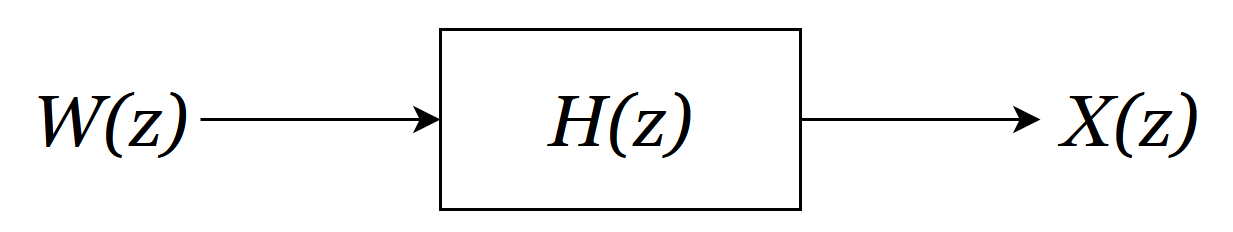
\includegraphics{BasicTF.png}
\caption{Basic Transfer Function}
\end{figure}

Here we have
\(W(z)\mathcal{H}(z) = X(z) \Rightarrow \mathcal{H}(z) = \frac{X(z)}{W(z)}\).
Therefore, in our case:

\[\frac{X(z)}{W(z)} = \frac{b_3}{1 + b_1 z^{-1} + b_2 z^{-2}} \Rightarrow  \mathcal{H}(z) = \frac{b_3}{1 + b_1 z^{-1} + b_2 z^{-2}}\]

Replacing the constants \(b_1\), \(b_2\) and \(b_3\) by the expressions
found in the previous question, we obtain:

\[\mathcal{H}(z) = \frac{b_3}{1 + b_1 z^{-1} + b_2 z^{-2}} \Leftrightarrow \mathcal{H}(z) = \frac{(\Delta t)^2 \beta}{(1 + \gamma \Delta t + (\omega \Delta t)^2) - (2 + \gamma \Delta t) z^{-1} + z^{-2}}\]

    The poles can be found by calculating the roots of the denominator of
\(\mathcal{H}(z)\).

\[ z^2 + b1*z + b2 = 0 \Leftrightarrow z = \frac{-b_1 \pm \sqrt{b_1^2 - 4\times 1 \times  b_2}}{2 \times 1} \]

Replacing \(b_1\) and \(b_2\) by their numeric counterparts, we obtain:

\[z_1 = \frac{1000500}{1001009} + \frac{500\sqrt{35}}{1001009} i \hspace{2cm} z_2 = \frac{1000500}{1001009} - \frac{500\sqrt{35}}{1001009} i\]

If we approximate the fractions, we get:

\[z_1 = 0.999492 + 0.002955 i \hspace{2cm} z_2 = 0.999492 - 0.002955 i\]

    \begin{tcolorbox}[breakable, size=fbox, boxrule=1pt, pad at break*=1mm,colback=cellbackground, colframe=cellborder]
\prompt{In}{incolor}{8}{\boxspacing}
\begin{Verbatim}[commandchars=\\\{\}]
\PY{n}{coeff} \PY{o}{=} \PY{p}{[}\PY{l+m+mi}{1}\PY{p}{,} \PY{n}{b1}\PY{p}{,} \PY{n}{b2}\PY{p}{]}
\PY{n}{roots} \PY{o}{=} \PY{n}{np}\PY{o}{.}\PY{n}{roots}\PY{p}{(}\PY{n}{coeff}\PY{p}{)}
\PY{n+nb}{print}\PY{p}{(}\PY{l+s+s1}{\PYZsq{}}\PY{l+s+s1}{The roots of the system are:}\PY{l+s+s1}{\PYZsq{}}\PY{p}{)}
\PY{n+nb}{print}\PY{p}{(}\PY{l+s+s1}{\PYZsq{}}\PY{l+s+s1}{z1 = }\PY{l+s+s1}{\PYZsq{}} \PY{o}{+} \PY{n+nb}{str}\PY{p}{(}\PY{n}{roots}\PY{p}{[}\PY{l+m+mi}{0}\PY{p}{]}\PY{p}{)}\PY{p}{)}
\PY{n+nb}{print}\PY{p}{(}\PY{l+s+s1}{\PYZsq{}}\PY{l+s+s1}{z2 = }\PY{l+s+s1}{\PYZsq{}} \PY{o}{+} \PY{n+nb}{str}\PY{p}{(}\PY{n}{roots}\PY{p}{[}\PY{l+m+mi}{1}\PY{p}{]}\PY{p}{)}\PY{p}{)}
\end{Verbatim}
\end{tcolorbox}

    \begin{Verbatim}[commandchars=\\\{\}]
The roots of the system are:
z1 = (0.9994915130633193+0.0029550582377274406j)
z2 = (0.9994915130633193-0.0029550582377274406j)
    \end{Verbatim}

    The transfer function can be written in the following form

\$ \mathcal{H}(z) = b\_3 \frac{1}{(1 - z_1 z^{-1})}
\frac{1}{(1 - z_2 z^{-1})}\$,

which means that it is a multiplication of two geometrical series of the
form

\$ \frac{1}{1 - r} = \sum\_\{n=0\}\^{}\{\infty\} r\^{}n \$.

A geometrical series is convergent for \$ \textbar{} r \textbar\_2
\textless{} 1 \$. Given that both of the poles calculated above satisfy
this condition (where \$ \textbar{} r \textbar\_2 =
\sqrt{Re(r)^2 + Im(r)^2} \$ ), it can be concluded that the transfer
function is absolute summable. This, according to Lemma 2.6, is
necessary and sufficient to conclude that the system is BIBO stable.

    \hypertarget{question-4}{%
\subsection{Question 4}\label{question-4}}

Simulate the difference equation of question 2 for \(k = 3,\cdots ,N\)
using the initial conditions \(x(1) = x(2) = 0\). To do this you should
generate discrete white noise samples using
\texttt{numpy.random.randn()}.

Provide:

\begin{itemize}
\tightlist
\item
  \emph{the script used to generate \(N\) samples of \(x(k)\).}
  \textbf{1 point}
\item
  \emph{a plot of one realization of sequence \(x(k)\).} \textbf{1
  point}
\end{itemize}

    \hypertarget{answer-4}{%
\subsubsection{Answer 4}\label{answer-4}}

\emph{Insert the cells with your answer below.}

    \begin{tcolorbox}[breakable, size=fbox, boxrule=1pt, pad at break*=1mm,colback=cellbackground, colframe=cellborder]
\prompt{In}{incolor}{9}{\boxspacing}
\begin{Verbatim}[commandchars=\\\{\}]
\PY{n}{N} \PY{o}{=} \PY{l+m+mi}{10}\PY{o}{*}\PY{o}{*}\PY{l+m+mi}{4}
\PY{n}{x} \PY{o}{=} \PY{n}{np}\PY{o}{.}\PY{n}{zeros}\PY{p}{(}\PY{n}{N}\PY{o}{+}\PY{l+m+mi}{1}\PY{p}{)}
\PY{n}{w} \PY{o}{=} \PY{n}{np}\PY{o}{.}\PY{n}{zeros}\PY{p}{(}\PY{n}{N}\PY{o}{+}\PY{l+m+mi}{1}\PY{p}{)}

\PY{k}{for} \PY{n}{k} \PY{o+ow}{in} \PY{n+nb}{range}\PY{p}{(}\PY{l+m+mi}{2}\PY{p}{,}\PY{n}{N}\PY{o}{+}\PY{l+m+mi}{1}\PY{p}{)}\PY{p}{:}
    \PY{n}{w\PYZus{}k} \PY{o}{=} \PY{n}{np}\PY{o}{.}\PY{n}{random}\PY{o}{.}\PY{n}{randn}\PY{p}{(}\PY{p}{)}
    \PY{n}{x\PYZus{}k} \PY{o}{=} \PY{n}{b3} \PY{o}{*} \PY{n}{w\PYZus{}k} \PY{o}{\PYZhy{}} \PY{n}{b1} \PY{o}{*} \PY{n}{x}\PY{p}{[}\PY{n}{k}\PY{o}{\PYZhy{}}\PY{l+m+mi}{1}\PY{p}{]} \PY{o}{\PYZhy{}} \PY{n}{b2} \PY{o}{*} \PY{n}{x}\PY{p}{[}\PY{n}{k}\PY{o}{\PYZhy{}}\PY{l+m+mi}{2}\PY{p}{]}\PY{p}{;}
    \PY{n}{x}\PY{p}{[}\PY{n}{k}\PY{p}{]}\PY{o}{=}\PY{n}{x\PYZus{}k}
    \PY{n}{w}\PY{p}{[}\PY{n}{k}\PY{p}{]}\PY{o}{=}\PY{n}{w\PYZus{}k}

\PY{n}{time} \PY{o}{=} \PY{n}{np}\PY{o}{.}\PY{n}{linspace}\PY{p}{(}\PY{l+m+mi}{0}\PY{p}{,} \PY{n}{N}\PY{o}{*}\PY{n}{Delta\PYZus{}t}\PY{p}{,} \PY{n}{N}\PY{o}{+}\PY{l+m+mi}{1}\PY{p}{)}
\PY{n}{plt}\PY{o}{.}\PY{n}{plot}\PY{p}{(}\PY{n}{time} \PY{p}{,} \PY{n}{x}\PY{p}{)}
\PY{n}{plt}\PY{o}{.}\PY{n}{xlabel}\PY{p}{(}\PY{l+s+s2}{\PYZdq{}}\PY{l+s+s2}{Time [s]}\PY{l+s+s2}{\PYZdq{}}\PY{p}{)}
\PY{n}{plt}\PY{o}{.}\PY{n}{ylabel}\PY{p}{(}\PY{l+s+s2}{\PYZdq{}}\PY{l+s+s2}{Position [m]}\PY{l+s+s2}{\PYZdq{}}\PY{p}{)}
\end{Verbatim}
\end{tcolorbox}

            \begin{tcolorbox}[breakable, size=fbox, boxrule=.5pt, pad at break*=1mm, opacityfill=0]
\prompt{Out}{outcolor}{9}{\boxspacing}
\begin{Verbatim}[commandchars=\\\{\}]
Text(0, 0.5, 'Position [m]')
\end{Verbatim}
\end{tcolorbox}
        
    \begin{center}
    \adjustimage{max size={0.9\linewidth}{0.9\paperheight}}{output_20_1.png}
    \end{center}
    { \hspace*{\fill} \\}
    
    \hypertarget{question-5}{%
\subsection{Question 5}\label{question-5}}

Let us denote one realization of the solution of the difference equation
by \(x(k,\lambda)\) for \(\lambda = 1\) and the used white noise
sequence by ˜ \(w(k,1)\). Then the task is to generate \(L\)
realizations \(x(k,\lambda)\) for \(\lambda = 1,\cdots,L\), with each
realization generated for a different realization of the discrete time
white noise sequence ˜ \(w(k,\lambda)\).

provide:

\begin{itemize}
\tightlist
\item
  \emph{script use to generate \(L\) realizations of \(x(k,\lambda)\).}
  \textbf{1 point}
\item
  \emph{plot of all \(L\) realizations for \(L = 30\).} \textbf{1 point}
\end{itemize}

    \hypertarget{answer-5}{%
\subsubsection{Answer 5}\label{answer-5}}

\emph{Insert the cells with your answer below.}

    \begin{tcolorbox}[breakable, size=fbox, boxrule=1pt, pad at break*=1mm,colback=cellbackground, colframe=cellborder]
\prompt{In}{incolor}{18}{\boxspacing}
\begin{Verbatim}[commandchars=\\\{\}]
\PY{n}{L} \PY{o}{=} \PY{l+m+mi}{30}
\PY{n}{xL} \PY{o}{=} \PY{n}{np}\PY{o}{.}\PY{n}{zeros}\PY{p}{(}\PY{p}{(}\PY{n}{N}\PY{o}{+}\PY{l+m+mi}{1}\PY{p}{,} \PY{n}{L}\PY{o}{+}\PY{l+m+mi}{1}\PY{p}{)}\PY{p}{)}
\PY{n}{wL} \PY{o}{=} \PY{n}{np}\PY{o}{.}\PY{n}{zeros}\PY{p}{(}\PY{p}{(}\PY{n}{N}\PY{o}{+}\PY{l+m+mi}{1}\PY{p}{,} \PY{n}{L}\PY{o}{+}\PY{l+m+mi}{1}\PY{p}{)}\PY{p}{)}

\PY{k}{for} \PY{n}{l} \PY{o+ow}{in} \PY{n+nb}{range}\PY{p}{(}\PY{l+m+mi}{0}\PY{p}{,}\PY{n}{L}\PY{o}{+}\PY{l+m+mi}{1}\PY{p}{)}\PY{p}{:}
    \PY{k}{for} \PY{n}{k} \PY{o+ow}{in} \PY{n+nb}{range}\PY{p}{(}\PY{l+m+mi}{2}\PY{p}{,}\PY{n}{N}\PY{o}{+}\PY{l+m+mi}{1}\PY{p}{)}\PY{p}{:}
        \PY{n}{wL\PYZus{}k} \PY{o}{=} \PY{n}{np}\PY{o}{.}\PY{n}{random}\PY{o}{.}\PY{n}{randn}\PY{p}{(}\PY{p}{)}
        \PY{n}{xL\PYZus{}k} \PY{o}{=} \PY{n}{b3} \PY{o}{*} \PY{n}{wL\PYZus{}k} \PY{o}{\PYZhy{}} \PY{n}{b1} \PY{o}{*} \PY{n}{xL}\PY{p}{[}\PY{n}{k}\PY{o}{\PYZhy{}}\PY{l+m+mi}{1}\PY{p}{,} \PY{n}{l}\PY{p}{]} \PY{o}{\PYZhy{}} \PY{n}{b2} \PY{o}{*} \PY{n}{xL}\PY{p}{[}\PY{n}{k}\PY{o}{\PYZhy{}}\PY{l+m+mi}{2}\PY{p}{,} \PY{n}{l}\PY{p}{]}\PY{p}{;}
        \PY{n}{xL}\PY{p}{[}\PY{n}{k}\PY{p}{,}\PY{n}{l}\PY{p}{]}\PY{o}{=}\PY{n}{xL\PYZus{}k}
        \PY{n}{wL}\PY{p}{[}\PY{n}{k}\PY{p}{,}\PY{n}{l}\PY{p}{]}\PY{o}{=}\PY{n}{wL\PYZus{}k}
\end{Verbatim}
\end{tcolorbox}

    \begin{tcolorbox}[breakable, size=fbox, boxrule=1pt, pad at break*=1mm,colback=cellbackground, colframe=cellborder]
\prompt{In}{incolor}{15}{\boxspacing}
\begin{Verbatim}[commandchars=\\\{\}]
\PY{k}{for} \PY{n}{i} \PY{o+ow}{in} \PY{n+nb}{range}\PY{p}{(}\PY{l+m+mi}{0}\PY{p}{,}\PY{n}{L}\PY{o}{+}\PY{l+m+mi}{1}\PY{p}{)}\PY{p}{:}
    \PY{n}{plt}\PY{o}{.}\PY{n}{plot}\PY{p}{(}\PY{n}{time} \PY{p}{,} \PY{n}{xL}\PY{p}{,} \PY{n}{linewidth}\PY{o}{=}\PY{l+m+mf}{0.5}\PY{p}{)}
    \PY{n}{plt}\PY{o}{.}\PY{n}{xlabel}\PY{p}{(}\PY{l+s+s2}{\PYZdq{}}\PY{l+s+s2}{Time [s]}\PY{l+s+s2}{\PYZdq{}}\PY{p}{)}
    \PY{n}{plt}\PY{o}{.}\PY{n}{ylabel}\PY{p}{(}\PY{l+s+s2}{\PYZdq{}}\PY{l+s+s2}{Position [m]}\PY{l+s+s2}{\PYZdq{}}\PY{p}{)}
\end{Verbatim}
\end{tcolorbox}

    \begin{center}
    \adjustimage{max size={0.9\linewidth}{0.9\paperheight}}{output_24_0.png}
    \end{center}
    { \hspace*{\fill} \\}
    
    \hypertarget{question-6}{%
\subsection{Question 6}\label{question-6}}

Using the L realizations of the previous questions, estimate the mean
and variance of the stochastic process \(x(k)\). Here, you can use the
approximation

\[E[x(k)] \sim \frac{1}{L} \sum^{L}_{\lambda = 1} x(k, \lambda)\]

and a similar approximation for the variance, or use the available
built-in \texttt{numpy} commands.

Provide:

\begin{itemize}
\tightlist
\item
  \emph{A script to calculate the mean and variance.} \textbf{1 point}
\item
  \emph{A plot of the mean and the variance over time.} \textbf{1 point}
\end{itemize}

    \hypertarget{answer-6}{%
\subsubsection{Answer 6}\label{answer-6}}

    \begin{tcolorbox}[breakable, size=fbox, boxrule=1pt, pad at break*=1mm,colback=cellbackground, colframe=cellborder]
\prompt{In}{incolor}{19}{\boxspacing}
\begin{Verbatim}[commandchars=\\\{\}]
\PY{n}{Ex} \PY{o}{=} \PY{l+m+mi}{1}\PY{o}{/}\PY{n}{L} \PY{o}{*} \PY{n}{np}\PY{o}{.}\PY{n}{sum}\PY{p}{(}\PY{n}{xL}\PY{p}{,} \PY{n}{axis}\PY{o}{=}\PY{l+m+mi}{1}\PY{p}{)}
\PY{n}{Ex2} \PY{o}{=} \PY{l+m+mi}{1}\PY{o}{/}\PY{n}{L} \PY{o}{*} \PY{n}{np}\PY{o}{.}\PY{n}{sum}\PY{p}{(}\PY{n}{xL}\PY{o}{*}\PY{o}{*}\PY{l+m+mi}{2}\PY{p}{,} \PY{n}{axis}\PY{o}{=}\PY{l+m+mi}{1}\PY{p}{)}
\PY{n}{Var} \PY{o}{=} \PY{n}{Ex2} \PY{o}{\PYZhy{}} \PY{n}{Ex}\PY{o}{*}\PY{o}{*}\PY{l+m+mi}{2}

\PY{n}{BIVar} \PY{o}{=} \PY{n}{np}\PY{o}{.}\PY{n}{zeros}\PY{p}{(}\PY{n}{N}\PY{o}{+}\PY{l+m+mi}{1}\PY{p}{)}
\PY{n}{BIAvg} \PY{o}{=} \PY{n}{np}\PY{o}{.}\PY{n}{zeros}\PY{p}{(}\PY{n}{N}\PY{o}{+}\PY{l+m+mi}{1}\PY{p}{)}

\PY{k}{for} \PY{n}{i} \PY{o+ow}{in} \PY{n+nb}{range}\PY{p}{(}\PY{l+m+mi}{0}\PY{p}{,}\PY{l+m+mi}{10001}\PY{p}{)}\PY{p}{:}
    \PY{n}{BIVar}\PY{p}{[}\PY{n}{i}\PY{p}{]} \PY{o}{=}  \PY{n}{np}\PY{o}{.}\PY{n}{var}\PY{p}{(}\PY{n}{xL}\PY{p}{[}\PY{n}{i}\PY{p}{,}\PY{p}{:}\PY{p}{]}\PY{p}{)}
    \PY{n}{BIAvg}\PY{p}{[}\PY{n}{i}\PY{p}{]} \PY{o}{=}  \PY{n}{np}\PY{o}{.}\PY{n}{mean}\PY{p}{(}\PY{n}{xL}\PY{p}{[}\PY{n}{i}\PY{p}{,}\PY{p}{:}\PY{p}{]}\PY{p}{)}

\PY{n}{plt}\PY{o}{.}\PY{n}{figure}\PY{p}{(}\PY{l+m+mi}{1}\PY{p}{)}
\PY{n}{plt}\PY{o}{.}\PY{n}{plot}\PY{p}{(}\PY{n}{time}\PY{p}{,} \PY{n}{Ex}\PY{p}{,} \PY{n}{label}\PY{o}{=}\PY{l+s+s2}{\PYZdq{}}\PY{l+s+s2}{Expected Value}\PY{l+s+s2}{\PYZdq{}}\PY{p}{)}
\PY{n}{plt}\PY{o}{.}\PY{n}{plot}\PY{p}{(}\PY{n}{time}\PY{p}{,} \PY{n}{BIAvg}\PY{p}{,} \PY{n}{label}\PY{o}{=}\PY{l+s+s2}{\PYZdq{}}\PY{l+s+s2}{Expected Value (Built\PYZhy{}In Function)}\PY{l+s+s2}{\PYZdq{}}\PY{p}{)}
\PY{n}{plt}\PY{o}{.}\PY{n}{legend}\PY{p}{(}\PY{n}{loc}\PY{o}{=}\PY{l+s+s2}{\PYZdq{}}\PY{l+s+s2}{lower right}\PY{l+s+s2}{\PYZdq{}}\PY{p}{)}
\PY{n}{plt}\PY{o}{.}\PY{n}{xlabel}\PY{p}{(}\PY{l+s+s1}{\PYZsq{}}\PY{l+s+s1}{Time [s]}\PY{l+s+s1}{\PYZsq{}}\PY{p}{)}
\PY{n}{plt}\PY{o}{.}\PY{n}{ylabel}\PY{p}{(}\PY{l+s+s1}{\PYZsq{}}\PY{l+s+s1}{E[x]}\PY{l+s+s1}{\PYZsq{}}\PY{p}{)}

\PY{n}{plt}\PY{o}{.}\PY{n}{figure}\PY{p}{(}\PY{l+m+mi}{2}\PY{p}{)}
\PY{n}{plt}\PY{o}{.}\PY{n}{plot}\PY{p}{(}\PY{n}{time}\PY{p}{,} \PY{n}{Var}\PY{p}{,} \PY{n}{label}\PY{o}{=}\PY{l+s+s2}{\PYZdq{}}\PY{l+s+s2}{Variance}\PY{l+s+s2}{\PYZdq{}}\PY{p}{)}
\PY{n}{plt}\PY{o}{.}\PY{n}{plot}\PY{p}{(}\PY{n}{time}\PY{p}{,} \PY{n}{BIVar}\PY{p}{,} \PY{n}{label}\PY{o}{=}\PY{l+s+s2}{\PYZdq{}}\PY{l+s+s2}{Variance (Built\PYZhy{}In Function)}\PY{l+s+s2}{\PYZdq{}}\PY{p}{)}
\PY{n}{plt}\PY{o}{.}\PY{n}{legend}\PY{p}{(}\PY{n}{loc}\PY{o}{=}\PY{l+s+s2}{\PYZdq{}}\PY{l+s+s2}{lower right}\PY{l+s+s2}{\PYZdq{}}\PY{p}{)}
\PY{n}{plt}\PY{o}{.}\PY{n}{xlabel}\PY{p}{(}\PY{l+s+s1}{\PYZsq{}}\PY{l+s+s1}{Time [s]}\PY{l+s+s1}{\PYZsq{}}\PY{p}{)}
\PY{n}{plt}\PY{o}{.}\PY{n}{ylabel}\PY{p}{(}\PY{l+s+s1}{\PYZsq{}}\PY{l+s+s1}{Var[x]}\PY{l+s+s1}{\PYZsq{}}\PY{p}{)}
\end{Verbatim}
\end{tcolorbox}

            \begin{tcolorbox}[breakable, size=fbox, boxrule=.5pt, pad at break*=1mm, opacityfill=0]
\prompt{Out}{outcolor}{19}{\boxspacing}
\begin{Verbatim}[commandchars=\\\{\}]
Text(0, 0.5, 'Var[x]')
\end{Verbatim}
\end{tcolorbox}
        
    \begin{center}
    \adjustimage{max size={0.9\linewidth}{0.9\paperheight}}{output_27_1.png}
    \end{center}
    { \hspace*{\fill} \\}
    
    \begin{center}
    \adjustimage{max size={0.9\linewidth}{0.9\paperheight}}{output_27_2.png}
    \end{center}
    { \hspace*{\fill} \\}
    
    \hypertarget{question-7}{%
\subsection{Question 7}\label{question-7}}

Based on the results of the previous question, is the the stochastic
process \(x(k)\) WSS? Why or why not? \textbf{1 point}

    \hypertarget{answer-7}{%
\subsubsection{Answer 7}\label{answer-7}}

    Recalling the properties of the mean and variance of WSS processes, we
have:

\begin{itemize}
\tightlist
\item
  \emph{\(m(k) = m_x < \infty\)}
\item
  \(\sigma^2 = E[(x(n)-E[x(n)^2])] = E[x(n)^2] - E[x(n)]^2 = r_x(0) - m_x^2\)
\item
  \(\sigma^2 = c_x(0) < \infty\).
\end{itemize}

Firstly, we require m(k) to be constant and bounded. If we observe the
values obtained for \(E[x]\), we can see that they're not always
constant. However:

    \begin{tcolorbox}[breakable, size=fbox, boxrule=1pt, pad at break*=1mm,colback=cellbackground, colframe=cellborder]
\prompt{In}{incolor}{11}{\boxspacing}
\begin{Verbatim}[commandchars=\\\{\}]
\PY{n}{mean\PYZus{}Ex} \PY{o}{=} \PY{n+nb}{sum}\PY{p}{(}\PY{n}{Ex}\PY{p}{)}\PY{o}{/}\PY{n+nb}{len}\PY{p}{(}\PY{n}{Ex}\PY{p}{)}
\PY{n}{deviation\PYZus{}from\PYZus{}mean} \PY{o}{=} \PY{n}{Ex}\PY{o}{\PYZhy{}}\PY{n}{mean\PYZus{}Ex}
\PY{n}{percent\PYZus{}deviation} \PY{o}{=} \PY{n}{deviation\PYZus{}from\PYZus{}mean} \PY{o}{/} \PY{l+m+mi}{100}
\PY{n}{percent\PYZus{}deviation\PYZus{}str} \PY{o}{=} \PY{l+s+s2}{\PYZdq{}}\PY{l+s+si}{\PYZob{}:.5f\PYZcb{}}\PY{l+s+s2}{\PYZdq{}}\PY{o}{.}\PY{n}{format}\PY{p}{(}\PY{n+nb}{max}\PY{p}{(}\PY{n}{percent\PYZus{}deviation}\PY{p}{)}\PY{p}{)}
\PY{n+nb}{print}\PY{p}{(}\PY{l+s+s1}{\PYZsq{}}\PY{l+s+s1}{The maximum deviation from the mean value of E[x] is }\PY{l+s+s1}{\PYZsq{}} \PY{o}{+} \PY{n}{percent\PYZus{}deviation\PYZus{}str} \PY{o}{+} \PY{l+s+s1}{\PYZsq{}}\PY{l+s+s1}{\PYZpc{}}\PY{l+s+s1}{\PYZsq{}}\PY{p}{)}
\end{Verbatim}
\end{tcolorbox}

    \begin{Verbatim}[commandchars=\\\{\}]
The maximum deviation from the mean value of E[x] is 0.00011\%
    \end{Verbatim}

    This sort of deviation can be atributted to the errors caused by the
approximations used for \(\frac{d(\cdot)}{d t}\) and
\(\frac{d^2(\cdot)}{d t^2}\). Hence one can assume
\(E[x] \approx cte. \approx 0\). Therefore, the first property is met.

The third bullet point stated that the autocovariance at \(t=0\), which
is equal to the variance, should be finite. Looking at the plot, one can
conclude that the variance is finite as it does not blow up to infinity
anywhere within the 10 seconds of the simulation.

Furthermore, the variance of a WSS process should tend to a constant
value for BIBO stable systems. If the system is not BIBO stable, the
values for the mean and the variance would actually diverege for
different realizations. It has already been proven that the system is
BIBO stable, meaning its poles are within the unit circle. However, the
poles are very close to the unit circle boundary, a result of which can
be seen in the variance plot. The variance does rise above zero rapidly
and looks as though it could be oscillating around a constant value but
the amplitude is too large to conclude whether that is true. The
simulation should be repeated for larger numbers of realizations and/or
compared to theoretical values in order to be certain if the variance
tends to a constant value.

    \hypertarget{question-8}{%
\subsection{Question 8}\label{question-8}}

The mean and variance of the stochastic process \(x(t)\) can also be
calculated analytically. This leads to the following expressions,

\[ \mu_x (t) = e^{-\gamma t/2}\bigg( x_0 \cos(\omega' t) + \gamma x_0 \frac{\sin(\omega' t)}{2 \omega'} \bigg), \]

\[ \sigma^2_x (t) = \frac{\beta^2}{2\gamma \omega^2} + e^{-\gamma t} \bigg( \frac{\beta^2}{8\gamma \omega'^2 \omega^2} \bigg)
\big(  -4\omega^2 + \gamma^2 \cos(\omega' t) - 2\gamma \omega' \sin(2 \omega' t)\big). \]

Here, \(\omega'\) is another frequency parameter with the value
\(\omega' = \sqrt{\omega^2-\gamma^2/4}\), and \(x_0\) is the value of
\(x\) at time \(t = 0\)(note that in this case this value greatly
simplifies the expression). Compare the theoretical mean and variance
with the estimated ones from question \(6\) for different values of
\(L\).

provide:

\begin{itemize}
\tightlist
\item
  \emph{The script used to calculate the theoretical mean and variance.}
  \textbf{1 point}
\item
  \emph{A plot of both the theoretical mean and variance together with
  the estimated onces from question \(6\) as a function of time. Plot
  all four sequences in one plot. make three plots one for \(L = 30\),
  one for \(L = 300\), and one for \(L = 3000\).} \textbf{2 points}
\end{itemize}

    \hypertarget{answer-8}{%
\subsubsection{Answer 8}\label{answer-8}}

    \begin{tcolorbox}[breakable, size=fbox, boxrule=1pt, pad at break*=1mm,colback=cellbackground, colframe=cellborder]
\prompt{In}{incolor}{20}{\boxspacing}
\begin{Verbatim}[commandchars=\\\{\}]
\PY{n}{L\PYZus{}vec} \PY{o}{=} \PY{p}{(}\PY{l+m+mi}{30}\PY{p}{,} \PY{l+m+mi}{100}\PY{p}{,} \PY{l+m+mi}{1000}\PY{p}{)}

\PY{n}{Ex} \PY{o}{=} \PY{n}{np}\PY{o}{.}\PY{n}{zeros}\PY{p}{(}\PY{p}{(}\PY{n}{N}\PY{o}{+}\PY{l+m+mi}{1}\PY{p}{,} \PY{n+nb}{len}\PY{p}{(}\PY{n}{L\PYZus{}vec}\PY{p}{)}\PY{p}{)}\PY{p}{)}  \PY{c+c1}{\PYZsh{} Vector to hold the expected values of x for each L, calculated with the given formula.}
\PY{n}{Ex2} \PY{o}{=} \PY{n}{np}\PY{o}{.}\PY{n}{zeros}\PY{p}{(}\PY{p}{(}\PY{n}{N}\PY{o}{+}\PY{l+m+mi}{1}\PY{p}{,} \PY{n+nb}{len}\PY{p}{(}\PY{n}{L\PYZus{}vec}\PY{p}{)}\PY{p}{)}\PY{p}{)}  \PY{c+c1}{\PYZsh{} Vector to hold the expected values of x\PYZca{}2 for each L, calculated with the given formula.}
\PY{n}{Var} \PY{o}{=} \PY{n}{np}\PY{o}{.}\PY{n}{zeros}\PY{p}{(}\PY{p}{(}\PY{n}{N}\PY{o}{+}\PY{l+m+mi}{1}\PY{p}{,} \PY{n+nb}{len}\PY{p}{(}\PY{n}{L\PYZus{}vec}\PY{p}{)}\PY{p}{)}\PY{p}{)}  \PY{c+c1}{\PYZsh{} Vector to hold the variance of x for each L, calculated with the given formula.}

\PY{k}{for} \PY{n}{i} \PY{o+ow}{in} \PY{n+nb}{range} \PY{p}{(}\PY{l+m+mi}{0}\PY{p}{,}\PY{n+nb}{len}\PY{p}{(}\PY{n}{L\PYZus{}vec}\PY{p}{)}\PY{p}{)}\PY{p}{:}
    \PY{n}{L} \PY{o}{=} \PY{n}{L\PYZus{}vec}\PY{p}{[}\PY{n}{i}\PY{p}{]}
    \PY{n}{xL} \PY{o}{=} \PY{n}{np}\PY{o}{.}\PY{n}{zeros}\PY{p}{(}\PY{p}{(}\PY{n}{N}\PY{o}{+}\PY{l+m+mi}{1}\PY{p}{,} \PY{n}{L}\PY{o}{+}\PY{l+m+mi}{1}\PY{p}{)}\PY{p}{)}
    \PY{n}{wL} \PY{o}{=} \PY{n}{np}\PY{o}{.}\PY{n}{zeros}\PY{p}{(}\PY{p}{(}\PY{n}{N}\PY{o}{+}\PY{l+m+mi}{1}\PY{p}{,} \PY{n}{L}\PY{o}{+}\PY{l+m+mi}{1}\PY{p}{)}\PY{p}{)}

    \PY{k}{for} \PY{n}{l} \PY{o+ow}{in} \PY{n+nb}{range}\PY{p}{(}\PY{l+m+mi}{0}\PY{p}{,}\PY{n}{L}\PY{o}{+}\PY{l+m+mi}{1}\PY{p}{)}\PY{p}{:}
        \PY{k}{for} \PY{n}{k} \PY{o+ow}{in} \PY{n+nb}{range}\PY{p}{(}\PY{l+m+mi}{2}\PY{p}{,}\PY{n}{N}\PY{o}{+}\PY{l+m+mi}{1}\PY{p}{)}\PY{p}{:}
            \PY{n}{wL\PYZus{}k} \PY{o}{=} \PY{n}{np}\PY{o}{.}\PY{n}{random}\PY{o}{.}\PY{n}{randn}\PY{p}{(}\PY{p}{)}
            \PY{n}{xL\PYZus{}k} \PY{o}{=} \PY{n}{b3} \PY{o}{*} \PY{n}{wL\PYZus{}k} \PY{o}{\PYZhy{}} \PY{n}{b1} \PY{o}{*} \PY{n}{xL}\PY{p}{[}\PY{n}{k}\PY{o}{\PYZhy{}}\PY{l+m+mi}{1}\PY{p}{,} \PY{n}{l}\PY{p}{]} \PY{o}{\PYZhy{}} \PY{n}{b2} \PY{o}{*} \PY{n}{xL}\PY{p}{[}\PY{n}{k}\PY{o}{\PYZhy{}}\PY{l+m+mi}{2}\PY{p}{,} \PY{n}{l}\PY{p}{]}\PY{p}{;}
            \PY{n}{xL}\PY{p}{[}\PY{n}{k}\PY{p}{,}\PY{n}{l}\PY{p}{]}\PY{o}{=}\PY{n}{xL\PYZus{}k}
            \PY{n}{wL}\PY{p}{[}\PY{n}{k}\PY{p}{,}\PY{n}{l}\PY{p}{]}\PY{o}{=}\PY{n}{wL\PYZus{}k}

    \PY{n}{Ex}\PY{p}{[}\PY{p}{:}\PY{p}{,}\PY{n}{i}\PY{p}{]} \PY{o}{=} \PY{l+m+mi}{1}\PY{o}{/}\PY{n}{L} \PY{o}{*} \PY{n}{np}\PY{o}{.}\PY{n}{sum}\PY{p}{(}\PY{n}{xL}\PY{p}{,} \PY{n}{axis}\PY{o}{=}\PY{l+m+mi}{1}\PY{p}{)}
    \PY{n}{Ex2}\PY{p}{[}\PY{p}{:}\PY{p}{,}\PY{n}{i}\PY{p}{]} \PY{o}{=} \PY{l+m+mi}{1}\PY{o}{/}\PY{n}{L} \PY{o}{*} \PY{n}{np}\PY{o}{.}\PY{n}{sum}\PY{p}{(}\PY{n}{xL}\PY{o}{*}\PY{o}{*}\PY{l+m+mi}{2}\PY{p}{,} \PY{n}{axis}\PY{o}{=}\PY{l+m+mi}{1}\PY{p}{)}
    \PY{n}{Var}\PY{p}{[}\PY{p}{:}\PY{p}{,}\PY{n}{i}\PY{p}{]} \PY{o}{=} \PY{n}{Ex2}\PY{p}{[}\PY{p}{:}\PY{p}{,}\PY{n}{i}\PY{p}{]} \PY{o}{\PYZhy{}} \PY{n}{Ex}\PY{p}{[}\PY{p}{:}\PY{p}{,}\PY{n}{i}\PY{p}{]}\PY{o}{*}\PY{o}{*}\PY{l+m+mi}{2}
\end{Verbatim}
\end{tcolorbox}

    \begin{tcolorbox}[breakable, size=fbox, boxrule=1pt, pad at break*=1mm,colback=cellbackground, colframe=cellborder]
\prompt{In}{incolor}{21}{\boxspacing}
\begin{Verbatim}[commandchars=\\\{\}]
\PY{c+c1}{\PYZsh{} Calculation of the Theoretical values of E[x] and \PYZbs{}sigma\PYZca{}2.}
\PY{n}{omega\PYZus{}} \PY{o}{=} \PY{n}{math}\PY{o}{.}\PY{n}{sqrt}\PY{p}{(}\PY{n}{omega}\PY{o}{*}\PY{o}{*}\PY{l+m+mi}{2} \PY{o}{\PYZhy{}} \PY{n}{gamma}\PY{o}{*}\PY{o}{*}\PY{l+m+mi}{2}\PY{o}{/}\PY{l+m+mi}{4}\PY{p}{)}
\PY{n}{x0} \PY{o}{=} \PY{l+m+mi}{0}
\PY{n}{avg} \PY{o}{=} \PY{n}{np}\PY{o}{.}\PY{n}{zeros}\PY{p}{(}\PY{n}{N}\PY{o}{+}\PY{l+m+mi}{1}\PY{p}{)}
\PY{n}{sigma2} \PY{o}{=} \PY{n}{np}\PY{o}{.}\PY{n}{zeros}\PY{p}{(}\PY{n}{N}\PY{o}{+}\PY{l+m+mi}{1}\PY{p}{)}
\PY{n}{aprox\PYZus{}var} \PY{o}{=} \PY{n}{np}\PY{o}{.}\PY{n}{zeros}\PY{p}{(}\PY{n}{N}\PY{o}{+}\PY{l+m+mi}{1}\PY{p}{)}

\PY{k}{for} \PY{n}{k} \PY{o+ow}{in} \PY{n+nb}{range}\PY{p}{(}\PY{l+m+mi}{0}\PY{p}{,}\PY{n}{N}\PY{o}{+}\PY{l+m+mi}{1}\PY{p}{)}\PY{p}{:}
    \PY{n}{var1} \PY{o}{=} \PY{p}{(}\PY{n}{beta}\PY{o}{*}\PY{o}{*}\PY{l+m+mi}{2}\PY{p}{)}\PY{o}{/}\PY{p}{(}\PY{l+m+mi}{2}\PY{o}{*}\PY{n}{gamma}\PY{o}{*}\PY{n}{omega}\PY{o}{*}\PY{o}{*}\PY{l+m+mi}{2}\PY{p}{)}
    \PY{n}{var2} \PY{o}{=} \PY{n}{math}\PY{o}{.}\PY{n}{exp}\PY{p}{(}\PY{o}{\PYZhy{}}\PY{n}{gamma}\PY{o}{*}\PY{n}{k}\PY{o}{*}\PY{n}{Delta\PYZus{}t}\PY{p}{)}\PY{o}{*}\PY{p}{(}\PY{p}{(}\PY{n}{beta}\PY{o}{*}\PY{o}{*}\PY{l+m+mi}{2}\PY{p}{)}\PY{o}{/}\PY{p}{(}\PY{l+m+mi}{8}\PY{o}{*}\PY{n}{gamma}\PY{o}{*}\PY{p}{(}\PY{n}{omega\PYZus{}}\PY{o}{*}\PY{o}{*}\PY{l+m+mi}{2}\PY{p}{)}\PY{o}{*}\PY{p}{(}\PY{n}{omega}\PY{o}{*}\PY{o}{*}\PY{l+m+mi}{2}\PY{p}{)}\PY{p}{)}\PY{p}{)}
    \PY{n}{var3} \PY{o}{=} \PY{p}{(}\PY{o}{\PYZhy{}}\PY{l+m+mi}{4}\PY{o}{*}\PY{n}{omega}\PY{o}{*}\PY{o}{*}\PY{l+m+mi}{2} \PY{o}{+} \PY{p}{(}\PY{n}{gamma}\PY{o}{*}\PY{o}{*}\PY{l+m+mi}{2}\PY{p}{)}\PY{o}{*}\PY{n}{math}\PY{o}{.}\PY{n}{cos}\PY{p}{(}\PY{n}{omega\PYZus{}}\PY{o}{*}\PY{n}{Delta\PYZus{}t}\PY{o}{*}\PY{n}{k}\PY{p}{)}\PY{o}{\PYZhy{}}\PY{l+m+mi}{2}\PY{o}{*}\PY{n}{gamma}\PY{o}{*}\PY{n}{omega\PYZus{}}\PY{o}{*}\PY{n}{math}\PY{o}{.}\PY{n}{sin}\PY{p}{(}\PY{l+m+mi}{2}\PY{o}{*}\PY{n}{omega\PYZus{}}\PY{o}{*}\PY{n}{Delta\PYZus{}t}\PY{o}{*}\PY{n}{k}\PY{p}{)}\PY{p}{)}

    \PY{n}{sigma2}\PY{p}{[}\PY{n}{k}\PY{p}{]} \PY{o}{=} \PY{n}{var1} \PY{o}{+} \PY{n}{var2}\PY{o}{*}\PY{n}{var3}
    \PY{n}{avg}\PY{p}{[}\PY{n}{k}\PY{p}{]} \PY{o}{=} \PY{n}{math}\PY{o}{.}\PY{n}{exp}\PY{p}{(}\PY{o}{\PYZhy{}}\PY{n}{gamma}\PY{o}{*}\PY{n}{k}\PY{o}{*}\PY{n}{Delta\PYZus{}t}\PY{o}{/}\PY{l+m+mi}{2}\PY{p}{)}\PY{o}{*}\PY{p}{(}\PY{n}{x0}\PY{o}{*}\PY{n}{math}\PY{o}{.}\PY{n}{cos}\PY{p}{(}\PY{n}{omega\PYZus{}}\PY{o}{*}\PY{n}{k}\PY{o}{*}\PY{n}{Delta\PYZus{}t}\PY{p}{)} \PY{o}{+} \PY{n}{gamma}\PY{o}{*}\PY{n}{x0}\PY{o}{*}\PY{p}{(}\PY{n}{math}\PY{o}{.}\PY{n}{sin}\PY{p}{(}\PY{n}{omega\PYZus{}}\PY{o}{*}\PY{n}{k}\PY{o}{*}\PY{n}{Delta\PYZus{}t}\PY{p}{)}\PY{p}{)}\PY{o}{/}\PY{p}{(}\PY{l+m+mi}{2}\PY{o}{*}\PY{n}{omega\PYZus{}}\PY{p}{)}\PY{p}{)}
\end{Verbatim}
\end{tcolorbox}

    \begin{tcolorbox}[breakable, size=fbox, boxrule=1pt, pad at break*=1mm,colback=cellbackground, colframe=cellborder]
\prompt{In}{incolor}{22}{\boxspacing}
\begin{Verbatim}[commandchars=\\\{\}]
\PY{n}{plt}\PY{o}{.}\PY{n}{figure}\PY{p}{(}\PY{l+m+mi}{1}\PY{p}{)}
\PY{n}{plt}\PY{o}{.}\PY{n}{plot}\PY{p}{(}\PY{n}{time}\PY{p}{,} \PY{n}{Ex}\PY{p}{[}\PY{p}{:}\PY{p}{,}\PY{l+m+mi}{0}\PY{p}{]}\PY{p}{,} \PY{n}{label}\PY{o}{=}\PY{l+s+s2}{\PYZdq{}}\PY{l+s+s2}{Expected Value, L = 30}\PY{l+s+s2}{\PYZdq{}}\PY{p}{)}
\PY{n}{plt}\PY{o}{.}\PY{n}{plot}\PY{p}{(}\PY{n}{time}\PY{p}{,} \PY{n}{Ex}\PY{p}{[}\PY{p}{:}\PY{p}{,}\PY{l+m+mi}{1}\PY{p}{]}\PY{p}{,} \PY{n}{label}\PY{o}{=}\PY{l+s+s2}{\PYZdq{}}\PY{l+s+s2}{Expected Value, L = 100}\PY{l+s+s2}{\PYZdq{}}\PY{p}{)}
\PY{n}{plt}\PY{o}{.}\PY{n}{plot}\PY{p}{(}\PY{n}{time}\PY{p}{,} \PY{n}{Ex}\PY{p}{[}\PY{p}{:}\PY{p}{,}\PY{l+m+mi}{2}\PY{p}{]}\PY{p}{,} \PY{n}{label}\PY{o}{=}\PY{l+s+s2}{\PYZdq{}}\PY{l+s+s2}{Expected Value, L = 1000}\PY{l+s+s2}{\PYZdq{}}\PY{p}{)}

\PY{n}{plt}\PY{o}{.}\PY{n}{plot}\PY{p}{(}\PY{n}{time} \PY{p}{,} \PY{n}{avg}\PY{p}{,} \PY{n}{label}\PY{o}{=}\PY{l+s+s2}{\PYZdq{}}\PY{l+s+s2}{Expected Value (Theory)}\PY{l+s+s2}{\PYZdq{}}\PY{p}{)}
\PY{n}{plt}\PY{o}{.}\PY{n}{legend}\PY{p}{(}\PY{n}{loc}\PY{o}{=}\PY{l+s+s2}{\PYZdq{}}\PY{l+s+s2}{lower right}\PY{l+s+s2}{\PYZdq{}}\PY{p}{)}
\PY{n}{plt}\PY{o}{.}\PY{n}{xlabel}\PY{p}{(}\PY{l+s+s1}{\PYZsq{}}\PY{l+s+s1}{Time [s]}\PY{l+s+s1}{\PYZsq{}}\PY{p}{)}
\PY{n}{plt}\PY{o}{.}\PY{n}{ylabel}\PY{p}{(}\PY{l+s+s1}{\PYZsq{}}\PY{l+s+s1}{E[x]}\PY{l+s+s1}{\PYZsq{}}\PY{p}{)}

\PY{n}{plt}\PY{o}{.}\PY{n}{figure}\PY{p}{(}\PY{l+m+mi}{2}\PY{p}{)}
\PY{n}{plt}\PY{o}{.}\PY{n}{plot}\PY{p}{(}\PY{n}{time}\PY{p}{,} \PY{n}{Var}\PY{p}{[}\PY{p}{:}\PY{p}{,}\PY{l+m+mi}{0}\PY{p}{]}\PY{p}{,} \PY{n}{label}\PY{o}{=}\PY{l+s+s2}{\PYZdq{}}\PY{l+s+s2}{Variance, L = 30}\PY{l+s+s2}{\PYZdq{}}\PY{p}{)}
\PY{n}{plt}\PY{o}{.}\PY{n}{plot}\PY{p}{(}\PY{n}{time}\PY{p}{,} \PY{n}{Var}\PY{p}{[}\PY{p}{:}\PY{p}{,}\PY{l+m+mi}{1}\PY{p}{]}\PY{p}{,} \PY{n}{label}\PY{o}{=}\PY{l+s+s2}{\PYZdq{}}\PY{l+s+s2}{Variance, L = 100}\PY{l+s+s2}{\PYZdq{}}\PY{p}{)}
\PY{n}{plt}\PY{o}{.}\PY{n}{plot}\PY{p}{(}\PY{n}{time}\PY{p}{,} \PY{n}{Var}\PY{p}{[}\PY{p}{:}\PY{p}{,}\PY{l+m+mi}{2}\PY{p}{]}\PY{p}{,} \PY{n}{label}\PY{o}{=}\PY{l+s+s2}{\PYZdq{}}\PY{l+s+s2}{Variance, L = 1000}\PY{l+s+s2}{\PYZdq{}}\PY{p}{)}


\PY{n}{plt}\PY{o}{.}\PY{n}{plot}\PY{p}{(}\PY{n}{time}\PY{p}{,} \PY{n}{sigma2}\PY{p}{,} \PY{n}{label}\PY{o}{=}\PY{l+s+s2}{\PYZdq{}}\PY{l+s+s2}{Variance (Theory)}\PY{l+s+s2}{\PYZdq{}}\PY{p}{)}
\PY{n}{plt}\PY{o}{.}\PY{n}{legend}\PY{p}{(}\PY{n}{loc}\PY{o}{=}\PY{l+s+s2}{\PYZdq{}}\PY{l+s+s2}{lower right}\PY{l+s+s2}{\PYZdq{}}\PY{p}{)}
\PY{n}{plt}\PY{o}{.}\PY{n}{xlabel}\PY{p}{(}\PY{l+s+s1}{\PYZsq{}}\PY{l+s+s1}{Time [s]}\PY{l+s+s1}{\PYZsq{}}\PY{p}{)}
\PY{n}{plt}\PY{o}{.}\PY{n}{ylabel}\PY{p}{(}\PY{l+s+s1}{\PYZsq{}}\PY{l+s+s1}{Var[x]}\PY{l+s+s1}{\PYZsq{}}\PY{p}{)}
\end{Verbatim}
\end{tcolorbox}

            \begin{tcolorbox}[breakable, size=fbox, boxrule=.5pt, pad at break*=1mm, opacityfill=0]
\prompt{Out}{outcolor}{22}{\boxspacing}
\begin{Verbatim}[commandchars=\\\{\}]
Text(0, 0.5, 'Var[x]')
\end{Verbatim}
\end{tcolorbox}
        
    \begin{center}
    \adjustimage{max size={0.9\linewidth}{0.9\paperheight}}{output_37_1.png}
    \end{center}
    { \hspace*{\fill} \\}
    
    \begin{center}
    \adjustimage{max size={0.9\linewidth}{0.9\paperheight}}{output_37_2.png}
    \end{center}
    { \hspace*{\fill} \\}
    
    \hypertarget{question-9}{%
\subsection{Question 9}\label{question-9}}

How do the estimations of the mean and variance vary with respect to the
number of realizations \(L\)? \textbf{1 point}

    \hypertarget{answer-9}{%
\subsubsection{Answer 9}\label{answer-9}}

As we can see from the plots above, as the number of realizations
increases, the plots of the Mean and Variance get closer to the true
values.

This result makes sense because, as the number of realizations
increases, we also expect the influence of the stochastic process
\(w(k)\) to trend to the mean of this stochatistic process, \(E[x]=0\).
What this implies is that, as the number of realizations increases, the
plots of the Mean and Variance will tend to their true values.

    \hypertarget{question-10}{%
\subsection{Question 10}\label{question-10}}

Use the results from questions 6-9 and from question 3 to make a final
conclusion on whether the stochastic process \(x(k)\) is WSS or not,
with motivation. \textbf{2 points}

    \hypertarget{answer-10}{%
\subsubsection{Answer 10}\label{answer-10}}

WSS stochastic processes have a time invariant and finite mean, and a
finite constant variance. The mean has already been proven to be
constant in Question 7, which is again confirmed based on the results of
Question 8. With more realizations, the plot of the simulation
approaches the theoretical function (\(m_x = 0\)) more and more closely.
Regarding the variance of BIBO stable systems, its plot should rapidly
rise from zero to the same constant value for each simulation. Such
behavior is especially observed for systems with poles well within the
unit circle. The system examined in this assignment has poles that are
just on the verge of being on the unit circle, which means that the
variance may not converge to the constant value immediately. The
calculated theoretical function rises to a constant value in about 2s
and so do the simulations with large numbers of realizations. It can be
therefore concluded that a constant value is indeed achieved. To sum up,
based on the mean and the variance behavior of the system, it can be
concluded that the system is WSS.


    % Add a bibliography block to the postdoc
    
    
    
\end{document}
